\documentclass{standalone}
\usepackage{tikz}
\usepackage{siunitx} % pour \SI
\begin{document}
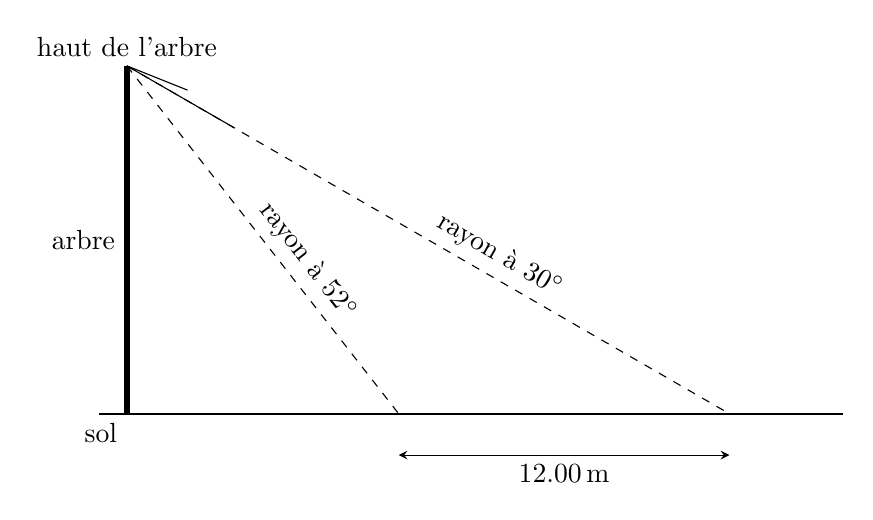
\begin{tikzpicture}[scale=0.35, >=stealth]
  % données numériques (arrondies pour le dessin)
  \def\h{12.62141298}    % hauteur de l'arbre en m (calculée)
  \def\sone{9.86092855}  % ombre quand le soleil est à 52°
  \def\stwo{21.86092855} % ombre quand le soleil est à 30°
  % sol
  \draw[thick] (-1,0) -- (26,0);
  % arbre (vertical)
  \draw[line width=2pt] (0,0) -- (0,\h) node[midway,left] {arbre};
  \draw (0,\h) node[above] {haut de l'arbre};
  % ombres sur le sol
  % rayons solaires depuis le sommet vers les points d'ombre
  \draw[dashed] (0,\h) -- (\sone,0) node[pos=0.6,above,sloped] {rayon à $52^\circ$};
  \draw[dashed] (0,\h) -- (\stwo,0) node[pos=0.6,above,sloped] {rayon à $30^\circ$};
  % angles au sommet projetés horizontalement (indication)
  % (on dessine de petits arcs d'angle près du sommet)
  \draw[thin] (0,\h) -- ++(2.2,-0.88); % repère direction horizontale
  \draw[thin] (0,\h) -- ++(3.9,-2.25); % repère direction 52°
  % annotation différence d'ombre
  \draw[<->] (\sone, -1.5) -- (\stwo, -1.5) node[midway,below] {$\SI{12.00}{m}$};
  % base
  \draw (0,0) node[below left] {sol};
  % échelle (optionnelle)

\end{tikzpicture}
\end{document}
